% --- SEKTION 3: ARCHITEKTUREN UND KOMPILIERUNG ---

\section{Vergleich ARM Cortex Architekturen}
\begin{description}
    \item[Cortex-A (Application):] Calcolo generico ad alte prestazioni (Linux/Android).
    \item[Cortex-R (Real-Time):] Bassa latenza e alta affidabilità (Automotive/Medicina).
    \item[Cortex-M (Microcontroller):] Consumo energetico ridotto, interrupt deterministici.
\end{description}

\renewcommand{\arraystretch}{1.5}
\resizebox{\columnwidth}{!}{
\begin{tabular}{|l|c|c|c|c|c|c|c|c|}
\hline
\textbf{Core} & \textbf{Thumb} & \textbf{Thumb-2} & \textbf{HW Mult.} & \textbf{HW Div.} & \textbf{Math Sat.} & \textbf{DSP} & \textbf{FPU} & \textbf{Arch} \\
\hline
Cortex-M0  & \cellcolor{green!60}Mostly & \cellcolor{green!60}Subset & \cellcolor{green!60}1/32 cyc & \cellcolor{red!60}No & \cellcolor{red!60}No & \cellcolor{red!60}No & \cellcolor{red!60}No & ARMv6-M \\
Cortex-M0+ & \cellcolor{green!60}Mostly & \cellcolor{green!60}Subset & \cellcolor{green!60}1/32 cyc & \cellcolor{red!60}No & \cellcolor{red!60}No & \cellcolor{red!60}No & \cellcolor{red!60}No & ARMv6-M \\
Cortex-M1  & \cellcolor{green!60}Mostly & \cellcolor{green!60}Subset & \cellcolor{green!60}3/33 cyc & \cellcolor{red!60}No & \cellcolor{red!60}No & \cellcolor{red!60}No & \cellcolor{red!60}No & ARMv6-M \\
Cortex-M3  & \cellcolor{green!60}Fully  & \cellcolor{green!60}Fully  & \cellcolor{green!60}1 cyc    & \cellcolor{green!60}Yes & \cellcolor{green!60}Yes & \cellcolor{red!60}No  & \cellcolor{red!60}No & 
ARMv7-M \\
Cortex-M4  & \cellcolor{green!60}Fully  & \cellcolor{green!60}Fully  & \cellcolor{green!60}1 cyc    & \cellcolor{green!60}Yes & \cellcolor{green!60}Yes & \cellcolor{green!60}Yes & \cellcolor{yellow!60}Optional & ARMv7E-M \\
Cortex-M7  & \cellcolor{green!60}Fully  & \cellcolor{green!60}Fully  & \cellcolor{green!60}1 cyc    & \cellcolor{green!60}Yes & \cellcolor{green!60}Yes & \cellcolor{green!60}Yes & \cellcolor{yellow!60}Optional & ARMv7E-M \\
\hline
\end{tabular}}
\renewcommand{\arraystretch}{1}

\subsection{Evolution Cortex-M0 vs M0+}
\begin{minipage}[t]{0.49\columnwidth}
    \begin{itemize}
        \item \textbf{Pipeline M0+:} Ridotta a 2 stadi per una maggiore efficienza.
        \item \textbf{Accesso I/O:} Supporto per GPIO a ciclo singolo.
        \item \textbf{Debugging:} Buffer di micro-traccia opzionale (MTB) per tracciare i salti.
    \end{itemize}
\end{minipage}\hfill
\begin{minipage}[t]{0.49\columnwidth}
    \textbf{Pipeline}
    \begin{itemize}
        \item[+] Viene eseguito un comando in ogni ciclo
        \item [-] In caso di salti, la pipeline deve essere "svuotata"
    \end{itemize}
    \textbf{MPU}
\end{minipage}


\section{Adressierungsarten ARM (Cortex-M0)}
\begin{minipage}{0.5\columnwidth}
    \begin{itemize}
        \item Registro diretto
        \item Registro indiretto
    \end{itemize}
\end{minipage}
\begin{minipage}{0.5\columnwidth}
    \begin{itemize}
        \item Registro indiretto con offset \texttt{[R?, \#imm]}
        \item Registro indiretto con indice \texttt{[R?, R?]}
    \end{itemize}
\end{minipage}

\begin{minipage}[t]{0.5\columnwidth}
    \subsection{Register Direkt, Immediate}
    \begin{itemize}
        \item \textbf{Immediate:} \texttt{MOV R0, \#100} $\rightarrow$ Il valore viene caricato direttamente.
        \item \textbf{Registro:} \texttt{MOVS R2, R1} $\rightarrow$ Copia il valore tra registri.
        \item \textbf{Vincoli:} I valori immediate vengono codificati nell'istruzione (ad es. 8-bit per \texttt{MOVS}).
    \end{itemize}

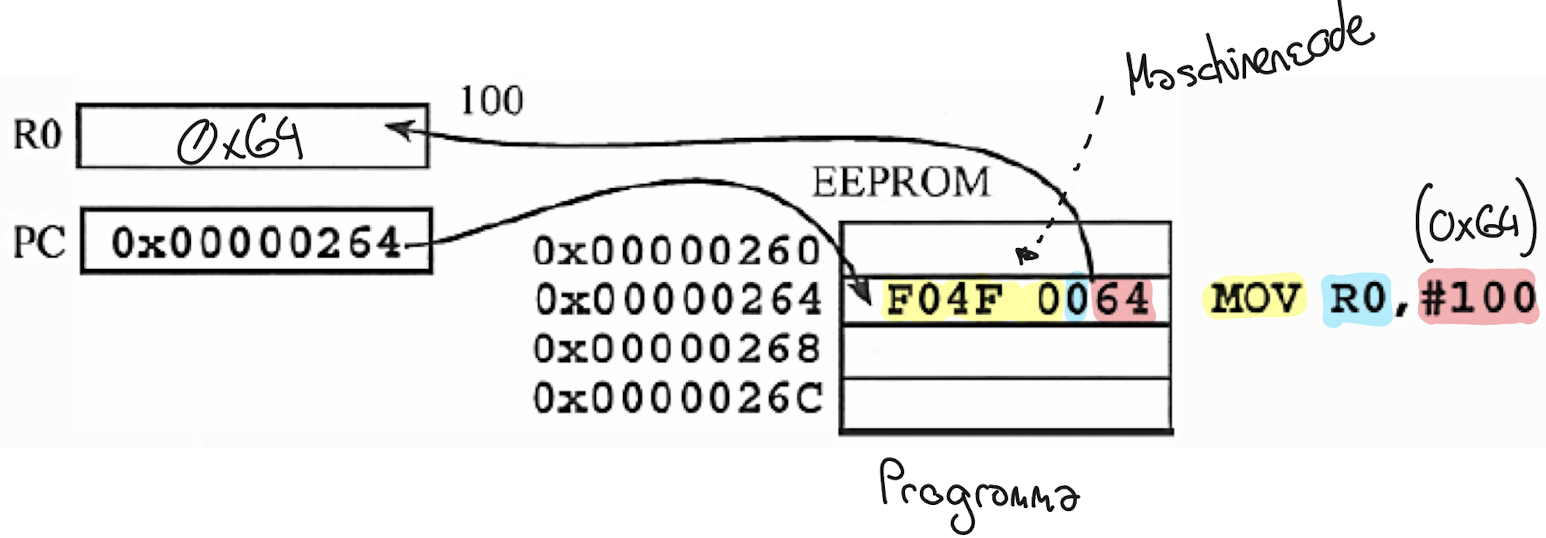
\includegraphics[width=\linewidth]{images/register_direkt.png}
\end{minipage}
\begin{minipage}[t]{0.5\columnwidth}
    \subsection{Register Indirekt (ptr)}
    \begin{itemize}
        \item \textbf{Semplice:} \texttt{LDR R0, [R1]} \\
        $\rightarrow$ $R0 = \text{valore all'indirizzo } R1$.
        \item \textbf{Con offset:} \texttt{LDR R0, [R1, \#4]} $\rightarrow$ $R0 = \text{valore all'indirizzo } R1 + 4$ (utile per array/struct).
        \item \textbf{Con indice:} \texttt{LDR R0, [R1, R2]} \\
        $\rightarrow$ $R0 = \text{valore all'indirizzo } R1 + R2$.
    \end{itemize}    
    \begin{center}
        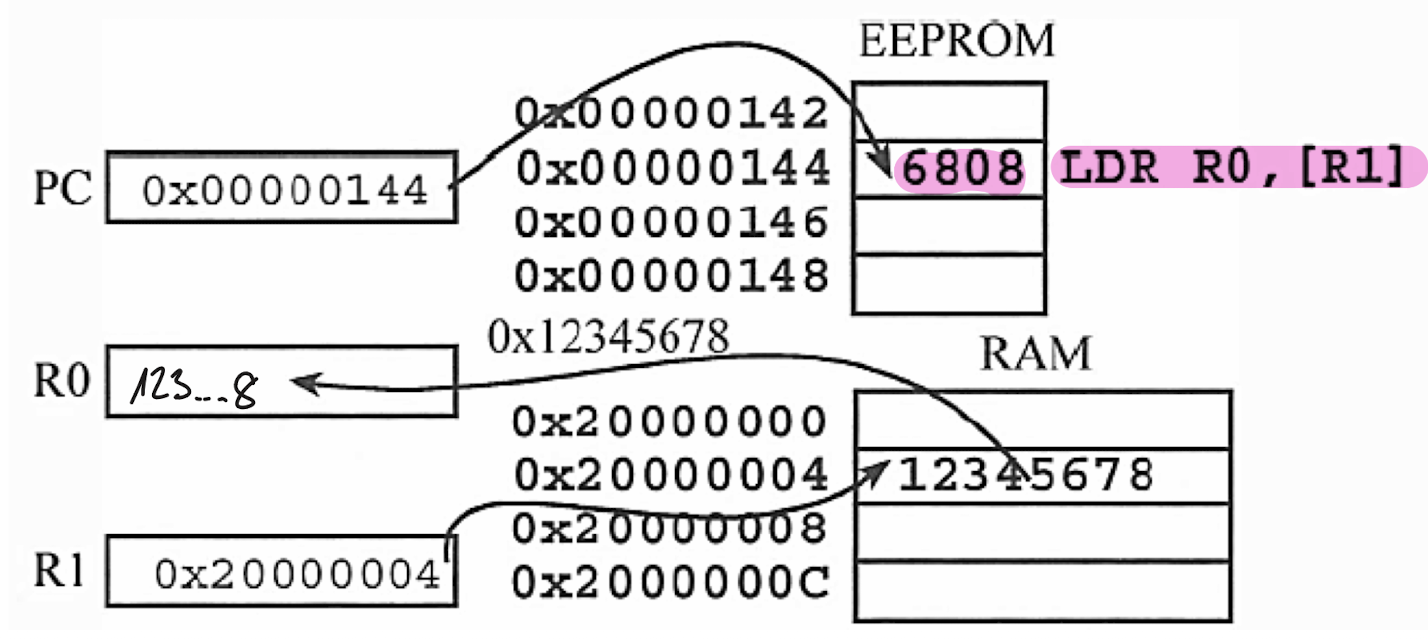
\includegraphics[width=\linewidth]{images/register_indirekt.png}
    \end{center}
\end{minipage}

\subsection{PC-Relative \& Literal Pool}
\begin{itemize}
    \item \textbf{Problema:} Le istruzioni a 32-bit non possono contenere costanti a 32-bit.
    \item \textbf{Soluzione:} L'assembler memorizza la costante nel \textbf{Literal Pool} (area di memoria in prossimità).
    \item \textbf{Accesso:} \texttt{LDR R0, =0x12345678} viene tradotto in \texttt{LDR R0, [PC, \#offset]}.
    \item Sono sempre necessari \textbf{due accessi alla memoria}
\end{itemize}

\subsection{Registerlisten \& Stack (SP-Relative)}
\begin{itemize}
    \item \textbf{Multiple:} \texttt{LDM R7!, \{R0-R3, R5\}} -> Carica più registri a partire dall'indirizzo contenuto in $R7$.
    \item \textbf{Stack:} \texttt{PUSH \{R0-R2\}}, \texttt{POP \{R0-R2\}}.
    \item \textbf{Regola d'oro:} Il registro con il numero più basso (\texttt{R0}) va sempre al più basso indirizzo di memoria.
    L'ordine tra le parentesi graffe non è rilevante per l'hardware.
\end{itemize}

\subsection{Stack Framing}
Il frame dello stack è l'area riservata in RAM per le variabili locali di una funzione.
\begin{minipage}{0.5\columnwidth}
    \begin{itemize}
        \item \textbf{Allocazione:} \texttt{SUB SP, SP, \#X} riserva $X$ byte (lo stack cresce verso indirizzi più bassi).
        \item \textbf{Frame Pointer ($R7$):} Si usa \texttt{MOV R7, SP} per avere un riferimento fisso all'inizio del frame.
        \item \textbf{Accesso:} Le variabili vengono scritte/lette usando offset relativi a $R7$, ad es.: \texttt{STR R0, [R7, \#4]}.
        \item \textbf{Deallocazione:} Prima del ritorno (\texttt{BX LR}) lo stack deve essere ripulito con \texttt{ADD SP, SP, \#X}.
    \end{itemize}
\end{minipage}
\begin{minipage}{0.5\columnwidth}
    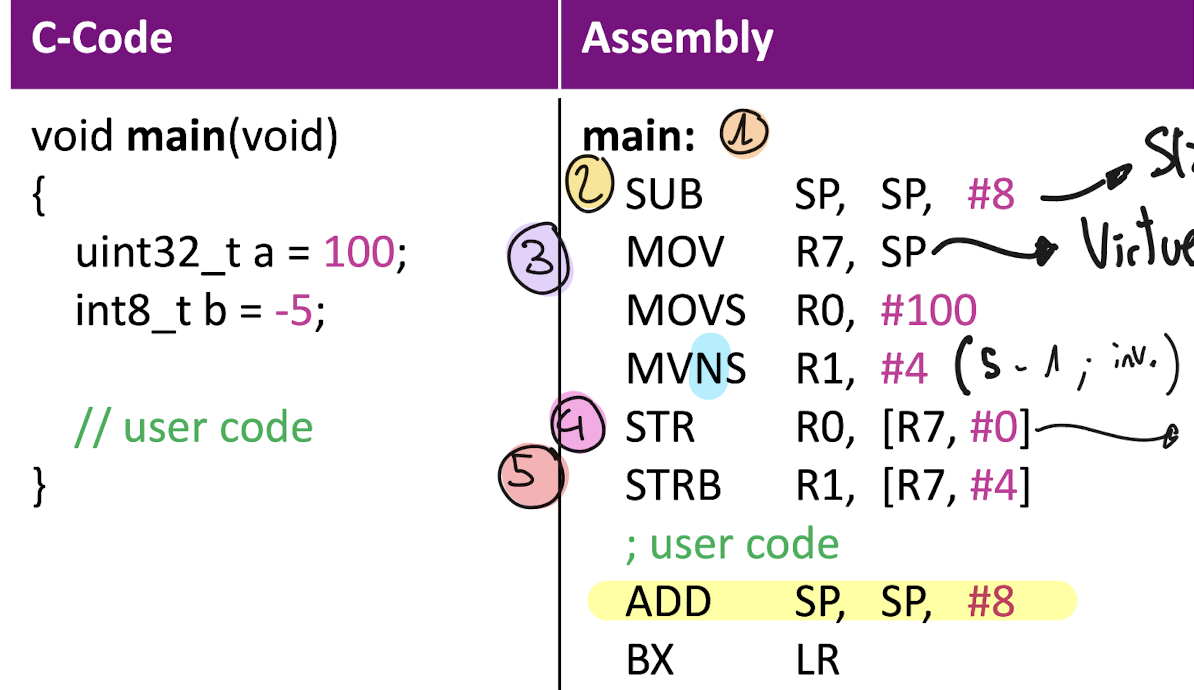
\includegraphics[width=\linewidth]{images/stack_framing.png}
\end{minipage}